\documentclass[10pt]{article}
\usepackage[margin=0.7in]{geometry}
\usepackage{enumitem}
\usepackage{tikz}
\usetikzlibrary{arrows.meta,positioning}

\setlist[itemize]{nosep,leftmargin=1.2em}
\setlength{\parindent}{0pt}
\setlength{\parskip}{5pt}

\title{\vspace{-2em}\textbf{Assignment 4}\\Building Resilient Distributed Systems}
\author{Abdul Basit \quad BSCS23023}
\date{}

\begin{document}
\maketitle
\vspace{-1.6em}

\section*{1. Problems in the Basic StudySync Design}

The main weakness in the first StudySync design is that it assumes every remote
service will behave like a local function call. In reality, the frontend,
FastAPI service, database, Clerk authentication system, and LLM provider all run
as separate networked components. Because of this, the system must be designed
for delays, duplicate requests, missed messages, and failures instead of assuming
that every operation will complete immediately and correctly.

\subsection*{1.1 Synchronization Problem}

The document editing bug is caused by a classic lost-update situation. Both users
load the same document state from the backend and begin editing from that old
copy. When they submit their changes, the backend accepts each request without
checking whether the document has already changed. As a result, the later
database write replaces the earlier one. The first user's work is lost not
because the database failed, but because the API has no version control,
conditional write, locking, or conflict-handling mechanism.

\subsection*{1.2 Coordination Problem}

The subscription problem happens because the app depends completely on a Clerk
webhook to update its own database. Clerk may know that a subscription was
cancelled, but the local application only changes its user record after receiving
and processing the webhook. If that HTTP request is dropped, times out, or fails
with a temporary server error, the application can continue treating the user as
premium. Without retry-safe processing, event storage, reconciliation, or a
dead-letter process, there is no reliable path for the missed cancellation to be
fixed.

\subsection*{1.3 Fault-Tolerance Problem}

The AI summary feature is fragile because the API waits directly for the external
LLM provider before replying to the user. If the provider becomes very slow, each
FastAPI worker remains blocked while waiting. When many users make requests at
the same time, these blocked workers can consume the available server capacity.
This can make the whole application feel unavailable even though only the LLM
dependency is unhealthy.

\section*{2. Improved Distributed-System Design}

\subsection*{2.1 Safer Document Editing with Optimistic Locking}

A better design is to attach a version number to every document. Each time a
client reads a document, the API also returns the current version. When the
client later sends an update, it must include the version it edited, such as in
an \texttt{If-Match} header. The backend then performs one atomic conditional
database update:

\texttt{UPDATE documents SET body=?, version=version+1 WHERE id=? AND version=?}

If the update changes one row, the client was editing the latest version and the
save succeeds. If no row is changed, another user has already saved a newer
version, so the API should return \texttt{409 Conflict}. The user can then reload,
compare changes, merge, or retry deliberately instead of silently overwriting
someone else's work.

\begin{center}
\resizebox{\textwidth}{!}{%
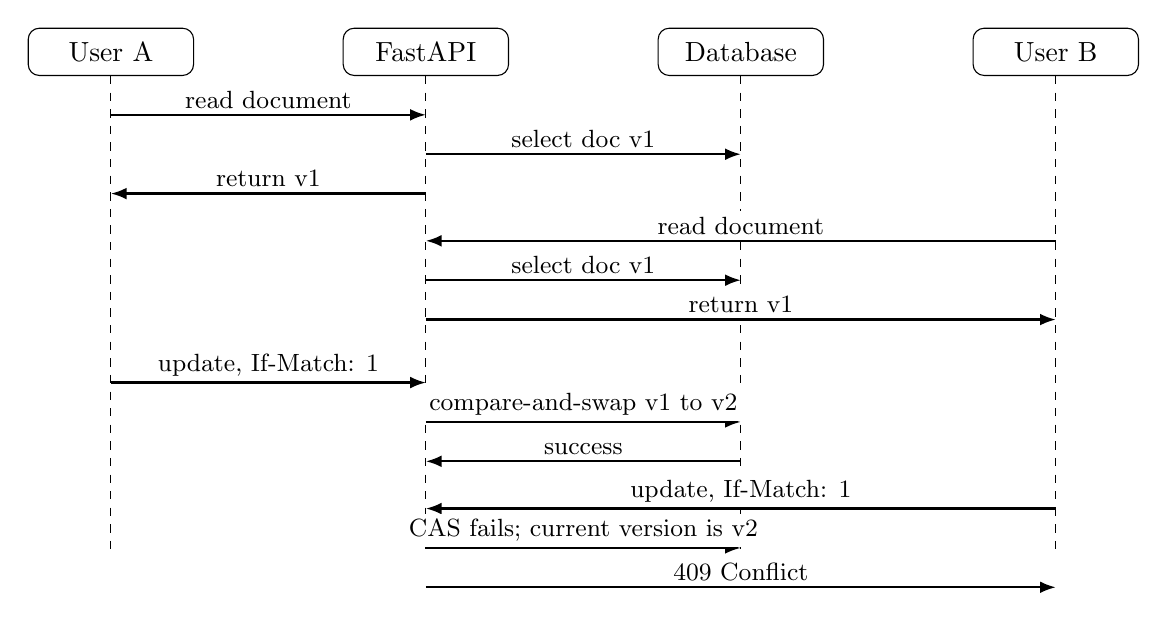
\begin{tikzpicture}[
  actor/.style={draw, rounded corners, minimum width=2.1cm, minimum height=.6cm},
  msg/.style={-{Latex[length=2mm]}, thick},
  note/.style={font=\small, fill=white, inner sep=2pt}
]
\node[actor] (a) at (0,0) {User A};
\node[actor] (api) at (4,0) {FastAPI};
\node[actor] (db) at (8,0) {Database};
\node[actor] (b) at (12,0) {User B};

\draw[dashed] (a) -- (0,-6.4);
\draw[dashed] (api) -- (4,-6.4);
\draw[dashed] (db) -- (8,-6.4);
\draw[dashed] (b) -- (12,-6.4);

\draw[msg] (0,-.8) -- node[note, above]{read document} (4,-.8);
\draw[msg] (4,-1.3) -- node[note, above]{select doc v1} (8,-1.3);
\draw[msg] (4,-1.8) -- node[note, above]{return v1} (0,-1.8);

\draw[msg] (12,-2.4) -- node[note, above]{read document} (4,-2.4);
\draw[msg] (4,-2.9) -- node[note, above]{select doc v1} (8,-2.9);
\draw[msg] (4,-3.4) -- node[note, above]{return v1} (12,-3.4);

\draw[msg] (0,-4.2) -- node[note, above]{update, If-Match: 1} (4,-4.2);
\draw[msg] (4,-4.7) -- node[note, above]{compare-and-swap v1 to v2} (8,-4.7);
\draw[msg] (8,-5.2) -- node[note, above]{success} (4,-5.2);

\draw[msg] (12,-5.8) -- node[note, above]{update, If-Match: 1} (4,-5.8);
\draw[msg] (4,-6.3) -- node[note, above]{CAS fails; current version is v2} (8,-6.3);
\draw[msg] (4,-6.8) -- node[note, above]{409 Conflict} (12,-6.8);
\end{tikzpicture}%
}
\end{center}


\subsection*{2.2 Reliable Subscription Updates Through Webhook Handling}

Webhook processing should be made durable and retry-safe. The backend should
first verify the Clerk signature, then store the event id and payload before
applying any business logic. The Clerk event id should be treated as an
idempotency key, so repeated deliveries of the same event do not cancel or modify
the account more than once.

If processing fails, the system should retry the event using exponential backoff.
After repeated failures, the event should be placed in a dead-letter queue so it
can be inspected, replayed, or handled manually. In addition, a scheduled
reconciliation job should compare the app's subscription records with Clerk's
current state. This ensures that even if a webhook is permanently missed, the
local database can eventually be corrected.

\subsection*{2.3 Protecting the API with a Circuit Breaker}

The LLM integration should not be allowed to block the whole application. The
FastAPI service should call the provider with short timeouts and monitor recent
failures. If the provider repeatedly times out or fails, the circuit breaker
should open. While it is open, the API should stop sending normal requests to the
LLM and immediately return a safe fallback, such as cached notes, a queued job
identifier, or a clear message that AI summaries are temporarily unavailable.

After a cooldown period, the circuit can move into a half-open state and allow a
small test request. If the test succeeds, normal traffic can resume. If it fails,
the circuit opens again. This keeps the unhealthy provider from consuming all API
capacity.

\section*{3. CAP-Based Design Choices}

StudySync does not need to make the same trade-off for every feature. For
collaborative document editing, consistency is more important than accepting
every write, so stale updates should be rejected with \texttt{409 Conflict}. This
protects user work even though it may require a reload or merge.

For subscription webhooks, the better approach is eventual consistency. The app
should accept events durably and process them asynchronously, using retries and
reconciliation to reach the correct state later.

For the LLM summary feature, availability and fast response matter more than
perfect freshness. If the AI provider is unhealthy, the system should keep the
main app responsive by returning fallbacks instead of waiting indefinitely.

\end{document}
